\documentclass[12pt, a4paper]{article}

% --- Language & Encoding ------------------------------------------------------
\usepackage[english]{babel}
\usepackage[T1]{fontenc}
\usepackage[utf8]{inputenc}

% --- Page Layout --------------------------------------------------------------
\usepackage[
  a4paper,
  top=2.5cm,
  bottom=2.5cm,
  left=3cm,
  right=3cm,
  marginparwidth=1.75cm
]{geometry}

% --- Typography ---------------------------------------------------------------
\usepackage{lmodern}
\usepackage{microtype}
\usepackage{setspace}
\onehalfspacing

% --- Mathematics --------------------------------------------------------------
\usepackage{amsmath}
\usepackage{amssymb}

% --- Graphics & Figures -------------------------------------------------------
\usepackage{graphicx}
\usepackage[labelfont=bf, font=small, skip=6pt]{caption}
\usepackage{float}
\usepackage{subcaption}

% --- Tables -------------------------------------------------------------------
\usepackage{booktabs}
\usepackage{array}
\usepackage{tabularx}
\usepackage{xcolor}
\usepackage{colortbl}
\usepackage{multirow}

% --- Headers & Footers --------------------------------------------------------
\usepackage{fancyhdr}
\pagestyle{fancy}
\fancyhf{}
\setlength{\headheight}{14pt}
\renewcommand{\headrulewidth}{0.4pt}
\fancyhead[L]{\small\textit{WSAI Summer Internship 2026}}
\fancyhead[R]{\small\textit{Project 2026/WSAI/029}}
\fancyfoot[C]{\thepage}

% --- Section Formatting -------------------------------------------------------
\usepackage{titlesec}
\titleformat{\section}{\large\bfseries}{{\thesection}}{1em}{}[\titlerule]
\titleformat{\subsection}{\normalsize\bfseries}{{\thesubsection}}{1em}{}
\titlespacing*{\section}{0pt}{16pt}{8pt}
\titlespacing*{\subsection}{0pt}{10pt}{4pt}

% --- Hyperlinks ---------------------------------------------------------------
\usepackage[
  colorlinks=true,
  linkcolor=blue!70!black,
  citecolor=blue!70!black,
  urlcolor=blue!70!black
]{hyperref}

% --- Miscellaneous ------------------------------------------------------------
\usepackage{parskip}
\setlength{\parskip}{6pt}
\usepackage{enumitem}

% --- Color Definitions --------------------------------------------------------
\definecolor{headerblue}{RGB}{36, 74, 116}
\definecolor{rowgray}{RGB}{240, 240, 240}
\definecolor{tpgreen}{RGB}{198, 239, 206}
\definecolor{tnblue}{RGB}{197, 217, 241}
\definecolor{fpred}{RGB}{255, 199, 206}
\definecolor{fnyellow}{RGB}{255, 235, 156}
\graphicspath{{figures/}}

\newcommand{\maybeincludegraphics}[2][]{%
  \IfFileExists{#2}{\includegraphics[#1]{#2}}{\fbox{\parbox[c][2.8cm][c]{4.5cm}{\centering Logo}}}%
}

\begin{document}
\hypersetup{pageanchor=false}

% --- Title Page ---------------------------------------------------------------
\begin{titlepage}
  \thispagestyle{empty}
  \centering

  \vspace*{0.25cm}

  \begin{minipage}[c]{0.22\textwidth}
    \centering
    
\includegraphics[height=2.25cm,keepaspectratio]{wsai_logo.png}
  \end{minipage}
  \hfill
  \begin{minipage}[c]{0.48\textwidth}
    \centering
    {\Large\bfseries Wadhwani School of Data Science and AI}\\[0.25em]
    {\large Indian Institute of Technology Madras}
  \end{minipage}
  \hfill
  \begin{minipage}[c]{0.22\textwidth}
    \centering
    
\includegraphics[height=2.25cm,keepaspectratio]{iitm_logo.png}
  \end{minipage}

  \vspace{0.45cm}
  \rule{0.78\textwidth}{0.5pt}

  \vspace{0.75cm}

  {\large\bfseries SUMMER INTERNSHIP REPORT}

  \vspace{0.75cm}

  {\LARGE\bfseries Multilingual Indic Text Embedding\\[0.4em]
   Model using Contrastive Learning}

  \vspace{0.65cm}

  {\itshape Submitted as part of the WSAI Summer Internship 2026 Programme}\\[0.5em]
  {\itshape Project ID: 2026/WSAI/029}

  \vspace{0.9cm}

  \begin{tabularx}{0.78\textwidth}{>{\bfseries}r >{\raggedright\arraybackslash}X}
    Project Title: & Multilingual Indic Text Embedding Model using Contrastive Learning\\
    Project ID: & 2026/WSAI/029\\
    Programme: & WSAI Summer Internship 2026\\
    Programme / Branch: & B.E. Computer Science and Engineering (AI\&ML)\\
    Project Area: & Multilingual Indic NLP, sentence embeddings, cross-lingual alignment\\
    Internship Period: & 11 May 2026 -- 12 June 2026
  \end{tabularx}

  \vspace{1.25cm}

  \begin{minipage}[t]{0.45\textwidth}
    \raggedright
    \textbf{Submitted by:}\\[0.4em]
    {\large\bfseries Surya Narayanaa}\\[0.3em]
    WSAI Summer Intern\\
    IIT Madras
  \end{minipage}
  \hfill
  \begin{minipage}[t]{0.47\textwidth}
    \raggedleft
    \textbf{Faculty in-charge:}\\[0.4em]
    {\large\bfseries Prof.\ B. Ravindran}\\[0.2em]
    {\large\bfseries Dr.\ Sudarsun Santhiappan}\\[0.3em]
    WSAI, IIT Madras
  \end{minipage}

  \vfill
  \rule{0.78\textwidth}{0.5pt}\\[0.4cm]
  {\large July 2026}
\end{titlepage}

\pagenumbering{roman}
\newpage
\thispagestyle{fancy}

\vspace*{0.18\textheight}

\begin{center}
{\Large\bfseries Acknowledgement}
\end{center}

\vspace{1cm}

I am deeply grateful to the Wadhwani School of Data Science and AI, IIT Madras for selecting me for the \textit{WSAI Summer Internship 2026} programme and for providing me with the opportunity to work on Project ID \textit{2026/WSAI/029}, titled \textit{``Multilingual Indic Text Embedding Model using Contrastive Learning''}. This internship allowed me to study practical embedding models, evaluate them systematically on Indic language pairs, and develop a fine-tuning workflow for improving LaBSE alignment across Indian languages.

\vspace{0.5em}

I sincerely thank Prof.\ B. Ravindran and Dr.\ Sudarsun Santhiappan, the faculty in-charge for this project, for their guidance, feedback, and support throughout the internship. I also thank the WSAI and IIT Madras teams for providing the computational environment and research setting required to conduct the benchmarking, training, and evaluation experiments reported here.

\vspace*{\fill}

\newpage

% --- Abstract -----------------------------------------------------------------
\begin{abstract}
\noindent
This report presents the work carried out for Project 2026/WSAI/029, \textit{``Multilingual Indic Text Embedding Model using Contrastive Learning''}, under the WSAI Summer Internship 2026 programme. The project studied sentence-level cross-lingual alignment for Indian languages, beginning with a literature survey of Indic NLP resources, Sentence-BERT, Contriever/mContriever, SimCSE, LaBSE, and Indic embedding models. It then developed benchmarking pipelines over FLORES-200, Samanantar, IN22-Gen, and IN22-Conv using retrieval metrics, cosine-separation metrics, and sensitivity/specificity diagnostics. These evaluations identified LaBSE as the most reliable overall baseline for Indic-Indic retrieval, while also showing that cosine similarity alone can be misleading when it is not paired with retrieval-based evaluation.

The final stage constructed a balanced all-pairs fine-tuning dataset for 22 Indic languages, covering 462 directed language pairs with 500 examples per pair. LaBSE was fine-tuned for five epochs using a contrastive sentence-pair objective and evaluated on a held-out IN22 conversion benchmark. The best all-462 fine-tuned model improved Accuracy@1 from 0.5654 to 0.5983, Recall@10 from 0.6816 to 0.7358, MRR from 0.6085 to 0.6511, and gold-random cosine gap from 0.3188 to 0.4002. These results show that balanced contrastive fine-tuning can improve direct Indic-Indic sentence alignment while preserving LaBSE as a strong multilingual embedding backbone.
\end{abstract}

\vspace{0.5em}

\newpage
\tableofcontents
\newpage
\pagenumbering{arabic}
\hypersetup{pageanchor=true}

% =============================================================================
\section{Problem Definition}
% =============================================================================

India's linguistic landscape contains many languages that differ in script, morphology, resource availability, and digital text coverage. Multilingual sentence embeddings are useful when text in one language must be compared directly with semantically equivalent text in another language. Such representations support cross-lingual semantic search, bitext mining, translation-memory retrieval, evaluation of machine translation outputs, multilingual question answering, and downstream NLP systems that must work across multiple Indian languages.

The central problem studied in this project is \textbf{Indic-Indic sentence alignment}: given a source sentence in one Indic language, retrieve the semantically corresponding target sentence from a candidate pool written in another Indic language. The task is evaluated using dense vector embeddings and cosine similarity. For a source sentence $s_i$ and target candidates $\{t_1,\ldots,t_n\}$, an embedding model $f(\cdot)$ maps each sentence to a vector. The retrieval score is:
\[
  \operatorname{sim}(s_i,t_j)
  =
  \frac{f(s_i)^\top f(t_j)}
       {\lVert f(s_i)\rVert_2 \lVert f(t_j)\rVert_2}.
\]
The correct target should rank as highly as possible among all candidates. The project therefore evaluates alignment through ranking metrics such as Accuracy@1, Recall@5, Recall@10, and Mean Reciprocal Rank (MRR), along with cosine-separation diagnostics.

\subsection{Project Objective}

The project objective is to benchmark multilingual embedding models for Indic sentence alignment and improve LaBSE for direct Indic-Indic retrieval. The specific goals are:

\begin{itemize}[leftmargin=1.5cm, itemsep=4pt]
  \item study sentence embedding and contrastive-learning literature relevant to Indic NLP;
  \item evaluate multiple multilingual embedding models on FLORES-200 and Samanantar alignment tasks;
  \item compare English-Indic and Indic-Indic alignment on IN22-Gen and IN22-Conv;
  \item compare threshold cosine, mean cosine, retrieval, cosine-gap, sensitivity, and specificity metrics;
  \item identify LaBSE's strengths and weaknesses across Indic language pairs;
  \item construct a balanced directed-pair training dataset covering 22 Indic languages;
  \item fine-tune LaBSE without relying on English as an intermediate pivot;
  \item evaluate the fine-tuned models on a held-out IN22 conversion benchmark; and
  \item analyse whether fine-tuning improves retrieval accuracy and cosine separation across language directions.
\end{itemize}

\subsection{Scope}

The project is sentence-level rather than document-level. It evaluates whether semantically equivalent sentences in different languages are placed near each other in embedding space and whether unrelated sentence pairs are kept sufficiently far apart. The work does not train a new encoder from scratch; instead, it evaluates pretrained multilingual and Indic-focused models, then fine-tunes LaBSE using contrastive sentence-pair objectives. The final experiments focus on direct Indic-Indic alignment across all 22 scheduled Indic languages.

\subsection{Languages and Directionality}

The final fine-tuning stage covers 22 languages: Assamese, Bengali, Bodo, Dogri, Gujarati, Hindi, Kannada, Kashmiri, Konkani, Maithili, Malayalam, Manipuri, Marathi, Nepali, Odia, Punjabi, Sanskrit, Santali, Sindhi, Tamil, Telugu, and Urdu. With 22 languages, the number of ordered source-target pairs excluding self-pairs is:
\[
  22 \times 21 = 462.
\]
Directionality matters because retrieval from language $a$ to language $b$ is not always equivalent to retrieval from $b$ to $a$. Tokenization quality, script coverage, sentence length, and corpus noise can affect each direction differently. For this reason, the dataset and evaluation treat pairs such as \texttt{hin->tam} and \texttt{tam->hin} as separate directed tasks.

\subsection{Baseline Model}

LaBSE, the Language-agnostic BERT Sentence Embedding model, was selected as the principal model for deeper study because the initial benchmarks showed that it was the strongest general-purpose multilingual alignment model among the tested candidates. LaBSE is trained for language-agnostic sentence representation and is widely used for bitext mining and cross-lingual retrieval. However, even strong multilingual models can show uneven behavior on low-resource or script-diverse Indic pairs. The project therefore investigates whether direct balanced fine-tuning over Indic-Indic pairs can improve the weaker directions while preserving broad alignment quality.

% =============================================================================
\section{Methodology}
% =============================================================================

\subsection{Literature Survey}

The initial phase of the internship was a focused literature survey covering Indic NLP resources, sentence embedding models, dense retrieval, and contrastive learning. This shaped both the model choices and the evaluation design.

\begin{table}[H]
\centering
\footnotesize
\renewcommand{\arraystretch}{1.2}
\begin{tabular}{>{\raggedright\arraybackslash}p{3.0cm} >{\raggedright\arraybackslash}p{4.8cm} >{\raggedright\arraybackslash}p{5.0cm}}
\toprule
\rowcolor{headerblue}
\textcolor{white}{\textbf{Topic}} &
\textcolor{white}{\textbf{Main Idea Studied}} &
\textcolor{white}{\textbf{Project Relevance}} \\
\midrule
\rowcolor{rowgray}
IndicBERT v2 / IndicCorp / IndicXTREME & Indic-specific corpora, benchmarks, and models for Indian languages. & Motivated all-Indic evaluation instead of relying only on global multilingual benchmarks. \\
Sentence-BERT & Siamese sentence encoders, pooling, cosine similarity, and sentence-level retrieval. & Provided the foundation for reusable sentence embeddings and pairwise similarity matrices. \\
\rowcolor{rowgray}
Contriever / mContriever & Dense retrieval with contrastive learning and in-batch negatives. & Informed retrieval-style evaluation and negative-pair interpretation. \\
SimCSE & Contrastive sentence representation, alignment, uniformity, and anisotropy. & Motivated reporting cosine gap and random-pair behavior, not only gold-pair cosine. \\
\rowcolor{rowgray}
LaBSE & Dual-encoder translation ranking with multilingual sentence embeddings. & Selected as the main baseline because its objective directly matches cross-lingual sentence retrieval. \\
\bottomrule
\end{tabular}
\caption{Literature survey themes and their connection to the project methodology.}
\label{tab:literature_survey}
\end{table}

\subsection{Repository and Experimental Workflow}

The project was organized around notebooks and exported scripts for benchmarking, data generation, fine-tuning, and evaluation. The workflow proceeded in five stages:

\begin{enumerate}[leftmargin=1.5cm, itemsep=4pt]
  \item \textbf{Literature and metric design:} study Indic NLP, sentence embeddings, contrastive learning, and alignment/uniformity.
  \item \textbf{Model benchmarking:} compare multilingual embedding models on FLORES and Samanantar retrieval tasks.
  \item \textbf{IN22 diagnostic evaluation:} measure English-Indic and Indic-Indic alignment over all 22 scheduled Indic languages.
  \item \textbf{Targeted pair fine-tuning:} study top-pair, bottom-pair, mixed-pair, and combined-pair LaBSE fine-tuning behavior.
  \item \textbf{Balanced all-pair fine-tuning:} train and evaluate the final all-462 directed-pair model on held-out IN22-Conv.
\end{enumerate}

The repository contains notebook groups for benchmarks, generation and baselines, directed-pair alignment, phase fine-tuning, model comparison, and final evaluation. The key reproducible artifacts include the reference list of 462 directed pairs, generated train and validation CSV files, training configuration files, epoch-wise training metrics, and IN22 evaluation summaries.

\subsection{Benchmarking Setup}

The initial benchmark evaluated sentence embedding models by encoding parallel sentence pairs and retrieving the correct translation using cosine similarity. The following model families were included in the benchmark stage:

\begin{itemize}[leftmargin=1.5cm, itemsep=4pt]
  \item \texttt{sentence-transformers/LaBSE};
  \item multilingual MPNet and MiniLM sentence-transformer models;
  \item MuRIL and IndicBERT-style Indic models;
  \item XLM-RoBERTa based embeddings;
  \item Contriever and multilingual Contriever variants; and
  \item supervised SimCSE variants and Vyakyarth in later IN22 comparisons.
\end{itemize}

For each model, source and target sentences were embedded independently. The target sentence with the highest cosine similarity to each source sentence was treated as the top-1 prediction. Ranking metrics were then computed over all sentence pairs in each language direction.

\subsection{Datasets and Evaluation Tracks}

The evaluation moved from clean multilingual benchmarks toward harder, broader Indic coverage. FLORES-200 provided clean multi-way alignment, Samanantar provided a noisier real-world comparison, and IN22-Gen/IN22-Conv enabled full coverage over all 22 scheduled Indic languages.

\begin{table}[H]
\centering
\footnotesize
\renewcommand{\arraystretch}{1.2}
\begin{tabular}{>{\raggedright\arraybackslash}p{3.1cm} >{\raggedright\arraybackslash}p{4.8cm} >{\raggedright\arraybackslash}p{5.0cm}}
\toprule
\rowcolor{headerblue}
\textcolor{white}{\textbf{Dataset / Track}} &
\textcolor{white}{\textbf{Coverage Used}} &
\textcolor{white}{\textbf{Role in Project}} \\
\midrule
\rowcolor{rowgray}
FLORES-200 & Clean multi-way aligned dev and devtest sentences. & Initial benchmark and clean Indic-Indic reference evaluation. \\
Samanantar & English-Indic samples and English-pivot inferred Indic-Indic pairs. & Stress-tested metric interpretation on noisier parallel data. \\
\rowcolor{rowgray}
IN22-Gen & 1,024 general-domain sentences over 22 scheduled Indic languages plus English. & General-domain full-language evaluation and source for earlier fine-tuning. \\
IN22-Conv & 1,503 conversational sentences over the same language set. & Harder held-out evaluation for baseline and fine-tuned models. \\
\rowcolor{rowgray}
Indic-Indic track & $22 \times 21 = 462$ directed pairs. & Main task: direct alignment between scheduled Indic languages. \\
English-Indic bidirectional track & 44 directions: English-to-Indic and Indic-to-English. & Reference track for comparing English-centered and direct Indic alignment. \\
\bottomrule
\end{tabular}
\caption{Datasets and evaluation tracks used across the internship experiments.}
\label{tab:datasets_tracks}
\end{table}

\subsection{Fine-Tuning Dataset}

The final training dataset was constructed for balanced direct Indic-Indic alignment. Each of the 462 directed language pairs contributed 500 sentence-pair examples, producing 231,000 rows before the train-validation split. A 90:10 split was used, resulting in 207,900 training rows and 23,100 validation rows.

\begin{table}[H]
\centering
\renewcommand{\arraystretch}{1.25}
\begin{tabular}{>{\raggedright\arraybackslash}p{6.5cm} >{\raggedright\arraybackslash}p{6cm}}
\toprule
\rowcolor{headerblue}
\textcolor{white}{\textbf{Dataset Property}} & \textcolor{white}{\textbf{Value}} \\
\midrule
\rowcolor{rowgray}
Base model & \texttt{sentence-transformers/LaBSE} \\
Number of Indic languages & 22 \\
\rowcolor{rowgray}
Directed language pairs & 462 \\
Examples per directed pair & 500 \\
\rowcolor{rowgray}
Total rows before split & 231,000 \\
Training rows & 207,900 \\
\rowcolor{rowgray}
Validation rows & 23,100 \\
Validation split & 10\% \\
\rowcolor{rowgray}
English pivot used & No \\
\bottomrule
\end{tabular}
\caption{Balanced all-462 directed-pair fine-tuning dataset.}
\label{tab:dataset}
\end{table}

The balanced construction was important because the objective was not only to improve high-resource directions such as Hindi, Bengali, Tamil, Telugu, or Marathi, but also to expose the model to difficult low-resource and script-sensitive directions involving languages such as Bodo, Manipuri, Santali, Sindhi, Kashmiri, and Dogri.

\subsection{Training Configuration}

LaBSE was fine-tuned using conservative hyperparameters to improve Indic alignment without destroying the model's original multilingual structure. The maximum sequence length was set to 128 tokens, the batch size was 32, and training ran for five epochs. The learning rate was $2 \times 10^{-6}$ with warmup and gradient clipping.

\begin{table}[H]
\centering
\renewcommand{\arraystretch}{1.25}
\begin{tabular}{p{6.5cm} p{6cm}}
\toprule
\rowcolor{headerblue}
\textcolor{white}{\textbf{Training Parameter}} & \textcolor{white}{\textbf{Value}} \\
\midrule
\rowcolor{rowgray}
Run name & All-pairs LaBSE fine-tuning \\
Maximum sequence length & 128 \\
\rowcolor{rowgray}
Batch size & 32 \\
Epochs & 5 \\
\rowcolor{rowgray}
Learning rate & $2 \times 10^{-6}$ \\
Warmup ratio & 0.1 \\
\rowcolor{rowgray}
Maximum gradient norm & 1.0 \\
Best checkpoint criterion & Validation cosine gap \\
\rowcolor{rowgray}
Checkpoint resume & Enabled \\
Epoch checkpoint saving & Enabled \\
\bottomrule
\end{tabular}
\caption{Fine-tuning configuration for the final balanced LaBSE run.}
\label{tab:training_config}
\end{table}

\subsection{Evaluation Metrics}

The main evaluation task is retrieval over candidate target sentences. The following metrics were used:

\textbf{Accuracy@1.}
The fraction of source sentences for which the correct target sentence is ranked first.
\[
  \operatorname{Accuracy@1}
  =
  \frac{1}{N}\sum_{i=1}^{N}\mathbf{1}[\operatorname{rank}_i = 1].
\]

\textbf{Recall@K.}
The fraction of examples for which the correct target appears within the top $K$ retrieved candidates. This report uses Recall@5 and Recall@10.
\[
  \operatorname{Recall@K}
  =
  \frac{1}{N}\sum_{i=1}^{N}\mathbf{1}[\operatorname{rank}_i \leq K].
\]

\textbf{Mean Reciprocal Rank.}
MRR rewards models that rank the correct target near the top even when it is not first.
\[
  \operatorname{MRR}
  =
  \frac{1}{N}\sum_{i=1}^{N}\frac{1}{\operatorname{rank}_i}.
\]

\textbf{Cosine Gap.}
The cosine gap measures separation between true translation pairs and randomly paired sentences:
\[
  \operatorname{CosineGap}
  =
  \operatorname{mean}(\cos_{\text{gold}})
  -
  \operatorname{mean}(\cos_{\text{random}}).
\]
A higher gap indicates stronger semantic separation and better suitability for retrieval.

\textbf{Sensitivity and Specificity at Midpoint.}
Gold-pair and random-pair cosine distributions were also evaluated with a midpoint decision threshold. Sensitivity measures how many true pairs are accepted; specificity measures how many random pairs are rejected. These are diagnostic metrics rather than the primary retrieval objective.

The reference report showed why these metrics must be interpreted together. Mean gold cosine alone can be misleading when random or wrong pairs also receive high similarity, as observed for some raw backbone models under simple mean pooling. Retrieval metrics answer whether the correct translation is ranked above alternatives, while cosine gap and sensitivity/specificity measure whether the embedding space separates true and wrong pairs in a usable way.

\newpage

% =============================================================================
\section{Experiments}
% =============================================================================

\subsection{FLORES-200 Model Benchmark}

The FLORES-200 benchmark provided a clean multilingual parallel corpus for comparing embedding models. In the all-pairs FLORES evaluation, LaBSE achieved the strongest alignment performance by a large margin, with Accuracy@1 of 0.9969, Recall@10 of 0.9986, and MRR of 0.9976. This confirmed that LaBSE was the best starting point for deeper Indic-specific work.

\begin{table}[H]
\centering
\scriptsize
\renewcommand{\arraystretch}{1.25}
\begin{tabular}{p{4.5cm} r r r r}
\toprule
\rowcolor{headerblue}
\textcolor{white}{\textbf{Model}} &
\textcolor{white}{\textbf{Acc@1}} &
\textcolor{white}{\textbf{Recall@10}} &
\textcolor{white}{\textbf{MRR}} &
\textcolor{white}{\textbf{Cosine Gap}} \\
\midrule
\rowcolor{rowgray}
LaBSE & 0.9969 & 0.9986 & 0.9976 & 0.5775 \\
MPNet multilingual & 0.7871 & 0.9076 & 0.8309 & 0.5710 \\
\rowcolor{rowgray}
MuRIL & 0.6310 & 0.8703 & 0.7134 & 0.0031 \\
SimCSE XLM-R multilingual & 0.4296 & 0.6992 & 0.5222 & 0.2886 \\
\rowcolor{rowgray}
mContriever & 0.2610 & 0.4661 & 0.3321 & 0.0960 \\
SBERT multilingual MiniLM & 0.2370 & 0.3291 & 0.2703 & 0.2273 \\
\bottomrule
\end{tabular}
\caption{Selected FLORES-200 all-pairs benchmark results.}
\label{tab:flores_benchmark}
\end{table}

\begin{figure}[H]
  \centering
  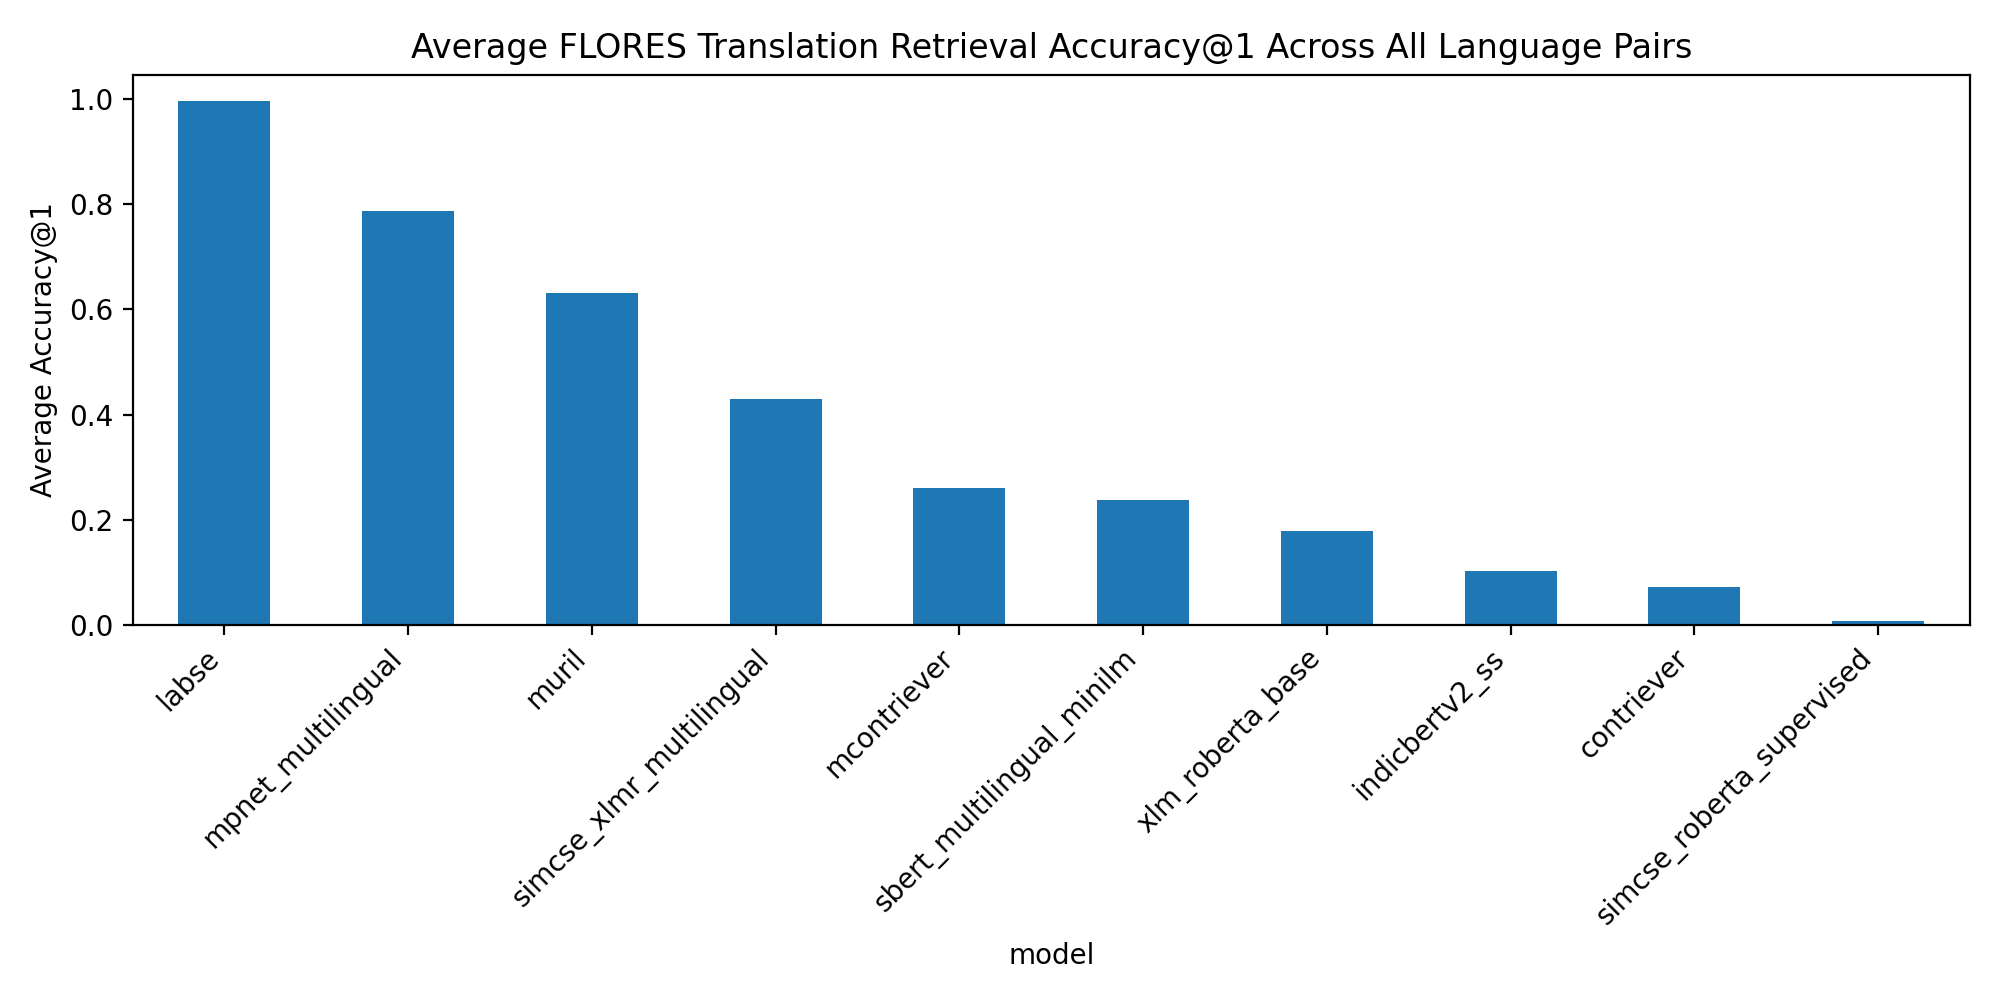
\includegraphics[width=0.94\linewidth]{flores_average_accuracy.png}
  \caption{Average FLORES-200 translation retrieval Accuracy@1 across model families.}
  \label{fig:flores_average_accuracy}
\end{figure}

\subsection{Samanantar Model Benchmark}

Samanantar is noisier and more domain-varied than FLORES-200, making it a useful stress test for cross-lingual alignment. LaBSE remained the strongest model, achieving Accuracy@1 of 0.9308 and Recall@10 of 0.9517. The gap between LaBSE and the next best model remained substantial, supporting the decision to focus the fine-tuning effort on LaBSE rather than switching to a weaker embedding backbone.

\begin{table}[H]
\centering
\footnotesize
\renewcommand{\arraystretch}{1.25}
\begin{tabular}{p{4.5cm} r r r r}
\toprule
\rowcolor{headerblue}
\textcolor{white}{\textbf{Model}} &
\textcolor{white}{\textbf{Acc@1}} &
\textcolor{white}{\textbf{Recall@10}} &
\textcolor{white}{\textbf{MRR}} &
\textcolor{white}{\textbf{Cosine Gap}} \\
\midrule
\rowcolor{rowgray}
LaBSE & 0.9308 & 0.9517 & 0.9392 & 0.5918 \\
MPNet multilingual & 0.6555 & 0.8295 & 0.7180 & 0.5296 \\
\rowcolor{rowgray}
MuRIL & 0.4985 & 0.7224 & 0.5774 & 0.0037 \\
SBERT multilingual MiniLM & 0.3200 & 0.4820 & 0.3771 & 0.3132 \\
\rowcolor{rowgray}
mContriever & 0.2107 & 0.4049 & 0.2775 & 0.0949 \\
IndicBERTv2 sentence similarity & 0.1122 & 0.1580 & 0.1305 & 0.0319 \\
\bottomrule
\end{tabular}
\caption{Selected Samanantar benchmark results.}
\label{tab:samanantar_benchmark}
\end{table}

\subsection{LaBSE Indic-Indic Diagnostic Benchmark}

Before fine-tuning, LaBSE was evaluated directly on Indic-Indic alignment data. On the dataset summaries available in the project artifacts, FLORES-200 produced a mean gold cosine of 0.8477 and Accuracy@1 of 0.9975, while the Samanantar English-pivot setting produced a mean gold cosine of 0.7877 and Accuracy@1 of 0.9130. These results show that LaBSE is highly capable, but also that alignment quality declines when the corpus is noisier and more realistic.

\begin{table}[H]
\centering
\renewcommand{\arraystretch}{1.25}
\begin{tabular}{p{4.8cm} r r r r}
\toprule
\rowcolor{headerblue}
\textcolor{white}{\textbf{Dataset}} &
\textcolor{white}{\textbf{Mean Gold Cos.}} &
\textcolor{white}{\textbf{Acc@1}} &
\textcolor{white}{\textbf{Recall@10}} &
\textcolor{white}{\textbf{MRR}} \\
\midrule
\rowcolor{rowgray}
FLORES-200 & 0.8477 & 0.9975 & 0.9992 & 0.9982 \\
Samanantar-EnglishPivot & 0.7877 & 0.9130 & 0.9619 & 0.9344 \\
\bottomrule
\end{tabular}
\caption{LaBSE Indic-Indic diagnostic dataset summary.}
\label{tab:labse_diagnostic}
\end{table}

\subsection{IN22 Model Comparison Reference}

The broader IN22 analysis in the reference report compared LaBSE with Vyakyarth and other multilingual baselines. Vyakyarth achieved a marginally higher cosine gap, but LaBSE remained stronger on retrieval metrics such as Accuracy@1 and Recall@10. This distinction is important because a model can have high gold-pair similarity or even strong cosine separation while still ranking the correct translation below competing candidates.

\begin{table}[H]
\centering
\scriptsize
\renewcommand{\arraystretch}{1.18}
\setlength{\tabcolsep}{3.5pt}
\begin{tabular}{>{\raggedright\arraybackslash}p{2.65cm} r r r r >{\raggedright\arraybackslash}p{2.75cm}}
\toprule
\rowcolor{headerblue}
\textcolor{white}{\textbf{Model}} &
\textcolor{white}{\textbf{Gold Cos.}} &
\textcolor{white}{\textbf{Random Cos.}} &
\textcolor{white}{\textbf{Gap}} &
\textcolor{white}{\textbf{Acc@1}} &
\textcolor{white}{\textbf{Interpretation}} \\
\midrule
\rowcolor{rowgray}
LaBSE & 0.5602 & 0.1704 & 0.3898 & 0.6544 & Best overall retrieval performer. \\
Vyakyarth & 0.4971 & 0.1062 & 0.3910 & 0.4937 & Highest gap, lower retrieval. \\
\rowcolor{rowgray}
MPNet multilingual & 0.5682 & 0.2340 & 0.3342 & 0.4046 & Strong general baseline. \\
MuRIL & 0.9868 & 0.9849 & 0.0018 & 0.2375 & High cosine, weak separation. \\
\rowcolor{rowgray}
XLM-RoBERTa base & 0.9928 & 0.9913 & 0.0015 & 0.0877 & Score inflation under mean pooling. \\
\bottomrule
\end{tabular}
\caption{IN22 Indic-Indic model comparison from the reference report.}
\label{tab:in22_model_comparison}
\end{table}

\begin{figure}[H]
  \centering
  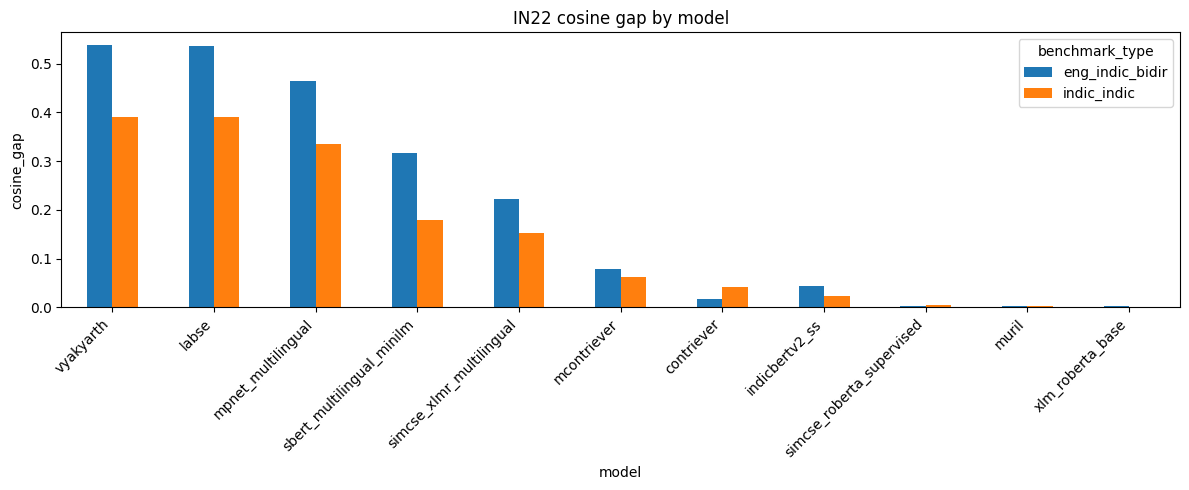
\includegraphics[width=0.92\linewidth]{in22_cosine_gap_by_model.png}
  \caption{IN22 cosine gap by model for English-Indic and Indic-Indic tracks.}
  \label{fig:in22_cosine_gap}
\end{figure}

\begin{figure}[H]
  \centering
  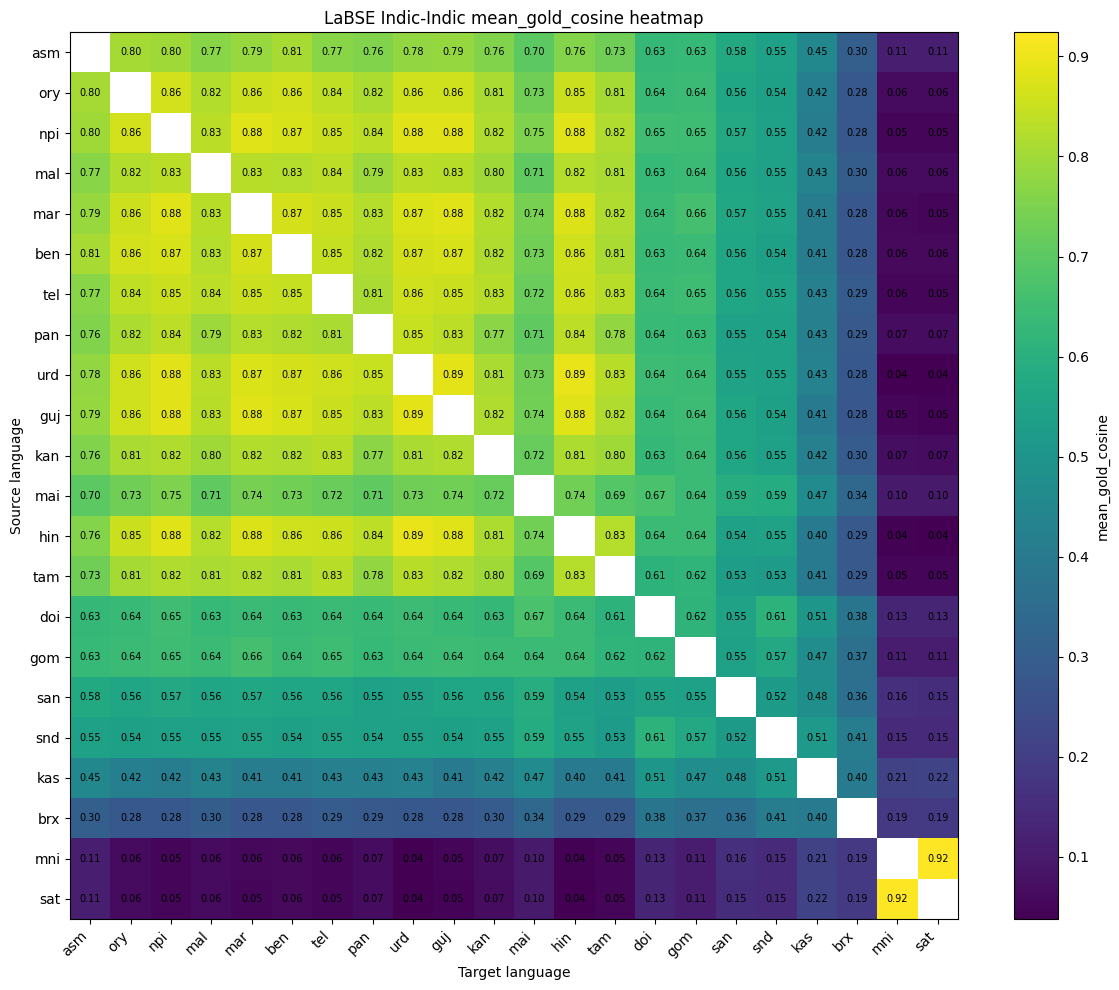
\includegraphics[width=0.86\linewidth]{labse_in22_mean_gold_cosine_heatmap.png}
  \caption{LaBSE IN22 Indic-Indic mean gold cosine heatmap. Lower-resource and script-specific languages such as Manipuri and Santali appear as weak regions.}
  \label{fig:labse_in22_heatmap}
\end{figure}

\subsection{Targeted Pair Fine-Tuning Reference}

Before the final all-pairs run, targeted LaBSE fine-tuning was explored on selected top-performing and bottom-performing directed pairs. The 13-model comparison showed that single-pair fine-tuning usually improved cosine gap over the LaBSE baseline, while combining several difficult bottom pairs in one small run degraded performance. This motivated the later balanced all-462 strategy: expose the model to all directions uniformly rather than over-concentrating on a small conflicting subset.

\begin{figure}[H]
  \centering
  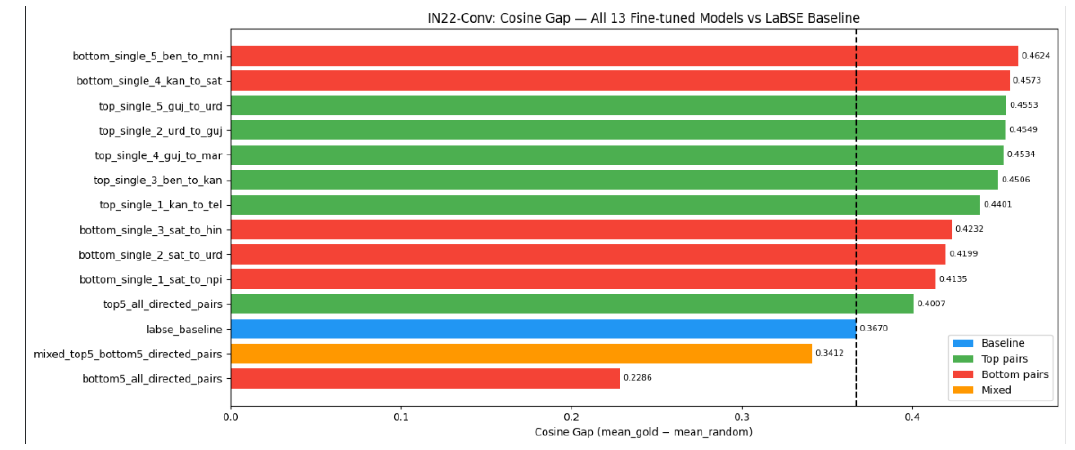
\includegraphics[width=0.95\linewidth]{finetuned_13model_cosine_gap.png}
  \caption{IN22-Conv cosine gap for 13 targeted fine-tuned LaBSE variants compared with the baseline.}
  \label{fig:targeted_finetuning}
\end{figure}

\subsection{Balanced All-462 Fine-Tuning}

The final experiment fine-tuned LaBSE on the balanced 462-pair dataset. The best checkpoint was selected using validation cosine gap. Over the five epochs, training loss decreased from 0.5315 to approximately 0.1886, while the validation cosine gap increased from 0.5909 to a peak of 0.6406 at epoch 4. This indicates that the model learned to separate true translation pairs from random pairs more effectively.

\begin{table}[H]
\centering
\footnotesize
\renewcommand{\arraystretch}{1.25}
\begin{tabular}{r r r r r}
\toprule
\rowcolor{headerblue}
\textcolor{white}{\textbf{Epoch}} &
\textcolor{white}{\textbf{Train Loss}} &
\textcolor{white}{\textbf{Gold Cos.}} &
\textcolor{white}{\textbf{Random Cos.}} &
\textcolor{white}{\textbf{Cosine Gap}} \\
\midrule
\rowcolor{rowgray}
1 & 0.5315 & 0.8034 & 0.2125 & 0.5909 \\
2 & 0.2674 & 0.7899 & 0.1706 & 0.6193 \\
\rowcolor{rowgray}
3 & 0.2143 & 0.7771 & 0.1422 & 0.6350 \\
4 & 0.1885 & 0.7662 & 0.1255 & 0.6406 \\
\rowcolor{rowgray}
5 & 0.1886 & 0.7701 & 0.1369 & 0.6332 \\
\bottomrule
\end{tabular}
\caption{Training and validation progress for the balanced all-462 LaBSE run.}
\label{tab:training_progress}
\end{table}

The validation trend is informative. Mean gold-pair cosine decreased slightly during training, but random-pair cosine decreased much more sharply. As a result, the net cosine gap increased. This is desirable for retrieval, because the model becomes more conservative about unrelated pairs while preserving relatively high similarity for true translations.

\newpage

% =============================================================================
\section{Results}
% =============================================================================

The final evaluation compared three models on the held-out IN22 conversion benchmark:

\begin{itemize}[leftmargin=1.5cm, itemsep=4pt]
  \item \textbf{LaBSE baseline:} the original \texttt{sentence-transformers/LaBSE} model;
  \item \textbf{All-462 best model:} the checkpoint selected by validation cosine gap; and
  \item \textbf{All-462 final model:} the checkpoint saved at the end of epoch 5.
\end{itemize}

\subsection{Overall IN22 Conversion Evaluation}

The best fine-tuned model improved every main retrieval metric over the LaBSE baseline. Accuracy@1 increased by 0.0329 absolute points, Recall@5 increased by 0.0474, Recall@10 increased by 0.0542, and MRR increased by 0.0426. The cosine gap increased from 0.3188 to 0.4002, showing better separation between true translation pairs and random pairs.

\begin{table}[H]
\centering
\footnotesize
\renewcommand{\arraystretch}{1.25}
\begin{tabular}{p{3.6cm} r r r r r}
\toprule
\rowcolor{headerblue}
\textcolor{white}{\textbf{Model}} &
\textcolor{white}{\textbf{Acc@1}} &
\textcolor{white}{\textbf{Recall@5}} &
\textcolor{white}{\textbf{Recall@10}} &
\textcolor{white}{\textbf{MRR}} &
\textcolor{white}{\textbf{Cosine Gap}} \\
\midrule
\rowcolor{rowgray}
LaBSE baseline & 0.5654 & 0.6523 & 0.6816 & 0.6085 & 0.3188 \\
All-462 best model & 0.5983 & 0.6997 & 0.7358 & 0.6511 & 0.4002 \\
\rowcolor{rowgray}
All-462 final model & 0.5974 & 0.6987 & 0.7351 & 0.6502 & 0.3938 \\
\bottomrule
\end{tabular}
\caption{Overall IN22 conversion evaluation by model.}
\label{tab:overall_results}
\end{table}

\begin{figure}[H]
  \centering
  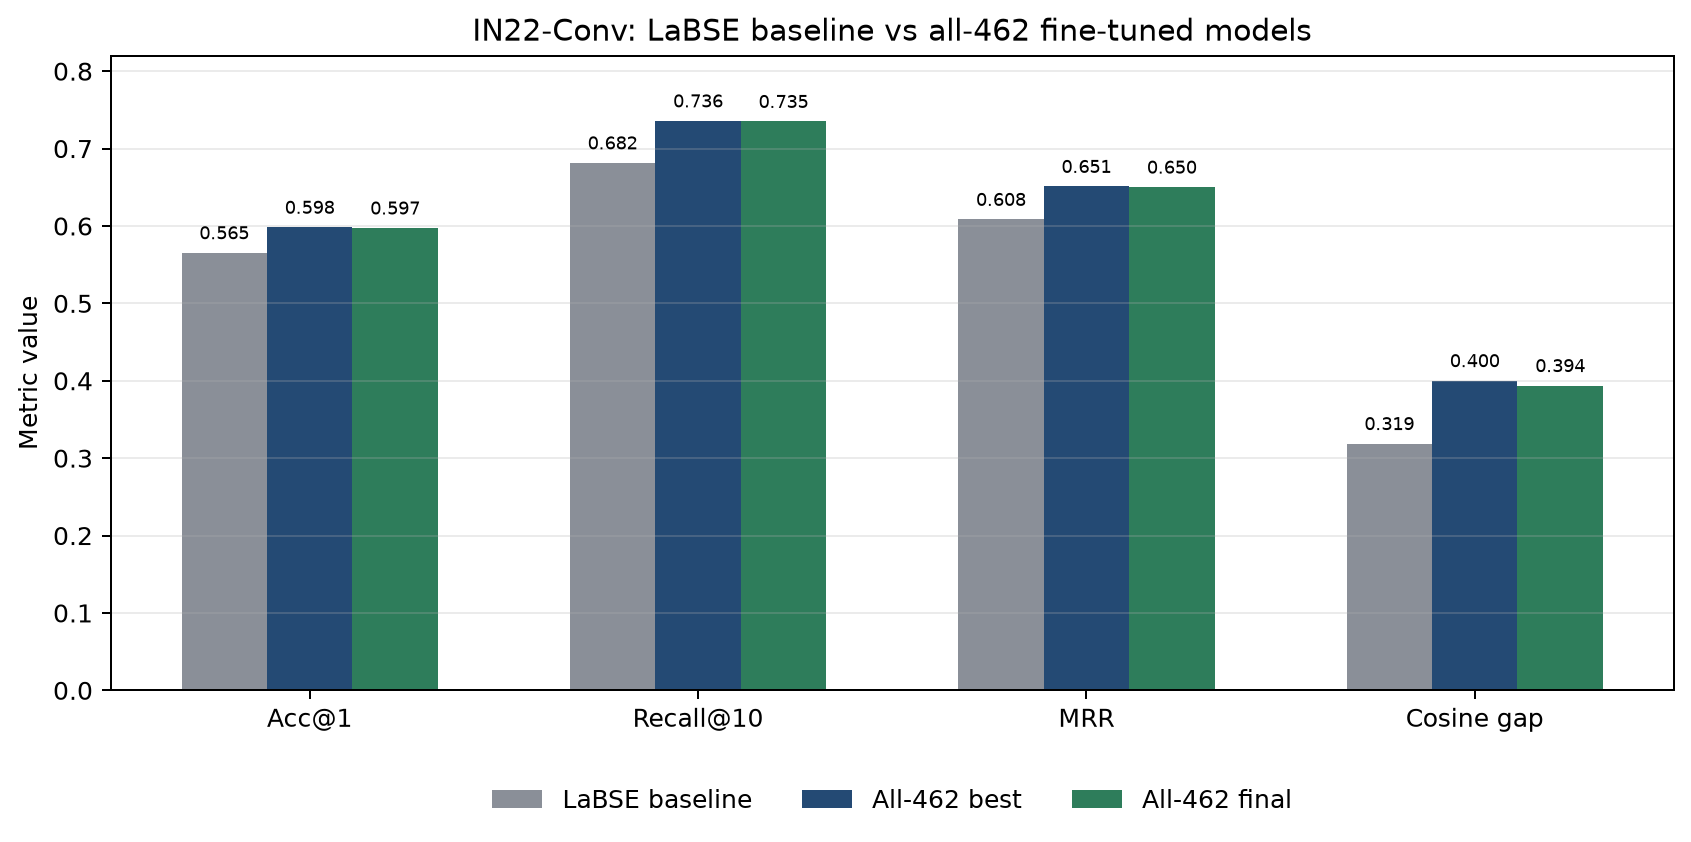
\includegraphics[width=0.92\linewidth]{all462_in22_metric_comparison.png}
  \caption{IN22-Conv comparison of LaBSE baseline, all-462 best checkpoint, and all-462 final checkpoint.}
  \label{fig:all462_metric_comparison}
\end{figure}

The best and final checkpoints are close in retrieval quality. The best checkpoint is marginally stronger on Accuracy@1, Recall@5, Recall@10, MRR, and cosine gap, so it is the preferred model for reporting and deployment.

\subsection{Improvement over Baseline}

\begin{table}[H]
\centering
\footnotesize
\renewcommand{\arraystretch}{1.25}
\begin{tabular}{p{3.3cm} r r r r r}
\toprule
\rowcolor{headerblue}
\textcolor{white}{\textbf{Model}} &
\textcolor{white}{\textbf{$\Delta$ Acc@1}} &
\textcolor{white}{\textbf{$\Delta$ Recall@5}} &
\textcolor{white}{\textbf{$\Delta$ Recall@10}} &
\textcolor{white}{\textbf{$\Delta$ MRR}} &
\textcolor{white}{\textbf{$\Delta$ Gap}} \\
\midrule
\rowcolor{rowgray}
All-462 best model & +0.0329 & +0.0474 & +0.0542 & +0.0426 & +0.0813 \\
All-462 final model & +0.0319 & +0.0464 & +0.0535 & +0.0417 & +0.0749 \\
\bottomrule
\end{tabular}
\caption{Absolute improvement over the LaBSE baseline on IN22 conversion evaluation.}
\label{tab:delta_results}
\end{table}

The most important gain is the increase in Recall@10. In practical retrieval and alignment workflows, top-k recall is valuable because downstream systems often inspect or rerank a shortlist rather than relying only on the single top prediction. A 0.0542 absolute gain in Recall@10 means that many more correct targets appear within a usable candidate set.

\subsection{Cosine Distribution Diagnostics}

The fine-tuned models substantially increased the mean cosine similarity of gold translation pairs. The baseline mean gold cosine was 0.5270, whereas the best model reached 0.7511. Random-pair cosine also increased from 0.2081 to 0.3510, but the increase for true pairs was larger, producing a net cosine-gap improvement.

\begin{table}[H]
\centering
\scriptsize
\renewcommand{\arraystretch}{1.25}
\begin{tabular}{p{3.2cm} r r r r r}
\toprule
\rowcolor{headerblue}
\textcolor{white}{\textbf{Model}} &
\textcolor{white}{\textbf{Gold Cos.}} &
\textcolor{white}{\textbf{Random Cos.}} &
\textcolor{white}{\textbf{Gap}} &
\textcolor{white}{\textbf{Sensitivity}} &
\textcolor{white}{\textbf{Specificity}} \\
\midrule
\rowcolor{rowgray}
LaBSE baseline & 0.5270 & 0.2081 & 0.3188 & 0.7877 & 0.8732 \\
All-462 best model & 0.7511 & 0.3510 & 0.4002 & 0.9220 & 0.8824 \\
\rowcolor{rowgray}
All-462 final model & 0.7569 & 0.3631 & 0.3938 & 0.9226 & 0.8811 \\
\bottomrule
\end{tabular}
\caption{Cosine-distribution diagnostics on IN22 conversion evaluation.}
\label{tab:cosine_diagnostics}
\end{table}

The sensitivity improvement is especially large, increasing from 0.7877 to 0.9220 for the best model. Specificity also improves slightly, indicating that the model does not merely raise all cosine scores indiscriminately; it improves true-pair acceptance while maintaining random-pair rejection.

\subsection{Language-Pair Behavior}

The per-direction results show that the fine-tuned model is most useful for weaker or more difficult language directions. For example, directions involving Bodo, Manipuri, Santali, Kashmiri, Sindhi, Dogri, and Sanskrit often show larger gains than already strong directions involving languages such as Bengali, Hindi, Marathi, Nepali, Gujarati, Odia, Tamil, or Telugu.

This pattern is expected. High-performing directions already start near saturation, leaving little room for Accuracy@1 improvement and sometimes showing small decreases because the model shifts capacity toward balanced all-pair alignment. In contrast, weaker directions benefit from explicit exposure during fine-tuning. The balanced design therefore behaves as intended: it raises the floor of multilingual retrieval performance rather than only optimizing the already strong languages.

\subsection{Best versus Final Checkpoint}

The final checkpoint is competitive but slightly below the best checkpoint on most retrieval metrics. The training-progress table explains this behavior: validation cosine gap peaks at epoch 4 and declines slightly at epoch 5. This suggests mild over-training after the best checkpoint. For submission and downstream use, the best checkpoint is therefore the preferred artifact.

\newpage

% =============================================================================
\section{Conclusion}
% =============================================================================

This project developed and evaluated a complete multilingual Indic text embedding workflow. The work began with broad model benchmarking, identified LaBSE as the strongest baseline, diagnosed Indic-Indic alignment behavior, constructed a balanced all-462 directed-pair dataset, fine-tuned LaBSE, and evaluated the resulting models on held-out IN22 conversion retrieval.

The earlier report and Notion-based work were also incorporated into this final account. They document the literature survey, FLORES and Samanantar pilots, IN22-Gen versus IN22-Conv comparison, Vyakyarth model comparison, and targeted top/bottom-pair fine-tuning experiments. Together, these stages show how the project evolved from simple cosine benchmarking into a more reliable contrastive-learning evaluation framework.

The final best model improved the LaBSE baseline on all major IN22 evaluation metrics:

\begin{itemize}[leftmargin=1.5cm, itemsep=4pt]
  \item \textbf{Accuracy@1} improved from 0.5654 to 0.5983.
  \item \textbf{Recall@5} improved from 0.6523 to 0.6997.
  \item \textbf{Recall@10} improved from 0.6816 to 0.7358.
  \item \textbf{MRR} improved from 0.6085 to 0.6511.
  \item \textbf{Cosine gap} improved from 0.3188 to 0.4002.
\end{itemize}

The results demonstrate that balanced direct fine-tuning across all directed Indic pairs can strengthen multilingual sentence alignment beyond the already strong LaBSE baseline. The improvement is particularly meaningful because the final evaluation was conducted on a held-out IN22 conversion benchmark rather than simply reusing the fine-tuning data. The project also shows that cosine-gap validation is a useful checkpoint-selection criterion: the best checkpoint slightly outperforms the final epoch checkpoint and should be used as the final model artifact.

Overall, the completed workflow provides a professional and reproducible foundation for Indic semantic search, parallel sentence retrieval, and downstream cross-lingual NLP applications.

% =============================================================================
\section{Limitations and Future Scope}
% =============================================================================

The experiments show clear gains, but several limitations remain.

\subsection{Limitations}

\textbf{Uneven pair-level performance.}
Although the overall metrics improve, individual language directions remain uneven. Low-resource languages and languages with script or corpus-quality challenges still show lower retrieval performance than high-resource directions.

\textbf{Risk of overfitting to benchmark distributions.}
The final model was trained and evaluated on curated aligned sentence data. Real-world retrieval may involve domain mismatch, noisy OCR, code-mixed text, transliteration, spelling variation, and sentence fragments that are not fully represented in the benchmark datasets.

\textbf{Limited model-family exploration during fine-tuning.}
The deeper fine-tuning work focused on LaBSE because it was the strongest baseline. Other architectures could potentially benefit from Indic-specific training, but they were not fine-tuned to the same depth in the final stage.

\textbf{Cosine score calibration.}
Fine-tuning increased both gold and random cosine means. Although the cosine gap improved, downstream applications that use fixed thresholds may need recalibration before adopting the fine-tuned model.

\begin{table}[H]
\centering
\footnotesize
\renewcommand{\arraystretch}{1.25}
\begin{tabular}{p{4.5cm} p{8.4cm}}
\toprule
\rowcolor{headerblue}
\textcolor{white}{\textbf{Limitation}} & \textcolor{white}{\textbf{Impact}} \\
\midrule
\rowcolor{rowgray}
Uneven language-pair performance & Some low-resource directions still require targeted improvement. \\
Benchmark distribution dependence & Real-world noisy text may reduce retrieval quality. \\
\rowcolor{rowgray}
Limited fine-tuned model families & LaBSE is validated most strongly; other backbones remain future work. \\
Threshold calibration & Applications using cosine cutoffs need validation after fine-tuning. \\
\bottomrule
\end{tabular}
\caption{Summary of limitations and practical impact.}
\label{tab:limitations}
\end{table}

\subsection{Future Scope}

\textbf{Targeted weak-pair fine-tuning.}
The next step is to continue training with higher sampling weight for the weakest directions while monitoring whether strong directions degrade. A curriculum that first learns broad balanced alignment and then focuses on difficult pairs may improve the performance floor.

\textbf{Hard-negative mining.}
Random negatives are useful but often too easy. Mining semantically close incorrect targets from the same language pair would force the model to learn finer distinctions and may improve top-1 retrieval.

\textbf{Domain robustness evaluation.}
The model should be tested on news, government documents, education content, social text, OCR outputs, and code-mixed inputs. This would measure whether benchmark gains transfer to realistic deployment settings.

\textbf{Threshold calibration and deployment packaging.}
For production semantic search or bitext mining, the model should be accompanied by calibrated thresholds per language pair, retrieval-speed benchmarks, model-card documentation, and examples of expected behavior.

\textbf{Comparison with modern embedding models.}
Future work can repeat the fine-tuning pipeline with newer multilingual sentence embedding backbones and compare them against the fine-tuned LaBSE model under the same IN22 evaluation protocol.

\newpage

% =============================================================================
\section*{References}
% =============================================================================

\begin{enumerate}[label={[\arabic*]}, itemsep=4pt, leftmargin=1.5cm]

  \item Feng, F., Yang, Y., Cer, D., Arivazhagan, N., and Wang, W. (2022).
        Language-agnostic BERT sentence embedding.
        \textit{Proceedings of the 60th Annual Meeting of the Association for Computational Linguistics}.

  \item Goyal, N., Gao, C., Chaudhary, V., Chen, P.-J., Wenzek, G., Ju, D., Krishnan, S., Ranzato, M., Guzman, F., and Fan, A. (2022).
        The FLORES-101 evaluation benchmark for low-resource and multilingual machine translation.
        \textit{Transactions of the Association for Computational Linguistics}, 10, 522--538.

  \item Team AI4Bharat. (2023).
        IN22: Indic language translation evaluation benchmark.
        \textit{AI4Bharat Dataset and Benchmark Resources}.

  \item Ramesh, G., Doddapaneni, S., Bheemaraj, A., Jobanputra, M., Ak, R., Sharma, A., Sahoo, S., Diddee, H., J, M., Kakwani, D., Kumar, N., Pradeep, A., Nagaraj, S., Deepak, K., Raghavan, V., Kunchukuttan, A., Kumar, P., and Khapra, M. M. (2022).
        Samanantar: The largest publicly available parallel corpora collection for 11 Indic languages.
        \textit{Transactions of the Association for Computational Linguistics}, 10, 145--162.

  \item Reimers, N. and Gurevych, I. (2019).
        Sentence-BERT: Sentence embeddings using Siamese BERT-networks.
        \textit{Proceedings of the 2019 Conference on Empirical Methods in Natural Language Processing}.

  \item Khanuja, S., Bansal, D., Mehtani, S., Khosla, S., Dey, A., Gopalan, B., Margam, D. K., Aggarwal, P., Nagipogu, R. T., Dave, S., Gupta, S., Gali, S. C. B., Subramanian, V., Talukdar, P., and Goyal, N. (2021).
        MuRIL: Multilingual representations for Indian languages.
        \textit{arXiv preprint arXiv:2103.10730}.

  \item Izacard, G., Caron, M., Hosseini, L., Riedel, S., Bojanowski, P., Joulin, A., and Grave, E. (2022).
        Unsupervised dense information retrieval with contrastive learning.
        \textit{Transactions on Machine Learning Research}.

  \item Gao, T., Yao, X., and Chen, D. (2021).
        SimCSE: Simple contrastive learning of sentence embeddings.
        \textit{Proceedings of EMNLP}.

  \item Internal project artifacts prepared during the internship:
        FLORES and Samanantar benchmark reports, IN22 alignment reports, LaBSE 13-model fine-tuning report, generated CSV metrics, plots, heatmaps, and notebook exports.

\end{enumerate}

\end{document}
